\documentclass[journal]{IEEEtran}

\usepackage[T1]{fontenc}
\usepackage[utf8]{inputenc}
\usepackage{amsmath,amssymb,amsfonts}
\usepackage{graphicx}
\usepackage{booktabs}
\usepackage{array}
\usepackage{longtable}
\usepackage{calc}
\usepackage{xcolor}
\usepackage{url}
\usepackage{cite}
\usepackage{tikz}
\usetikzlibrary{arrows.meta,positioning,calc,fit,backgrounds}

\graphicspath{{../}}

% ---- shared tikz styles for the architecture schematic ----
\tikzset{
  blk/.style={draw,rounded corners=2pt,align=center,font=\footnotesize,
              minimum height=8mm,inner sep=3pt,fill=blue!4},
  det/.style={draw,rounded corners=2pt,align=center,font=\footnotesize,
              minimum height=8mm,inner sep=3pt,fill=orange!10},
  offb/.style={draw,dashed,rounded corners=2pt,align=center,font=\footnotesize,
              minimum height=8mm,inner sep=3pt,fill=green!6},
  sig/.style={-{Latex[length=2mm]},line width=0.6pt},
  dot/.style={circle,fill,inner sep=1.1pt}
}

% shrink a display equation to the column width only if it would otherwise overflow
\newcommand{\eqfit}[1]{\resizebox{\ifdim\width>\columnwidth \columnwidth\else \width\fi}{!}{\ensuremath{\displaystyle #1}}}

\providecommand{\texorpdfstring}[2]{#1}
\DeclareUnicodeCharacter{2248}{\ensuremath{\approx}}
\DeclareUnicodeCharacter{2022}{\textbullet}

\newcounter{none}
\providecommand{\tightlist}{%
  \setlength{\itemsep}{0pt}\setlength{\parskip}{0pt}}

\makeatletter
\newsavebox\pandoc@box
\newcommand*\pandocbounded[1]{%
  \sbox\pandoc@box{#1}%
  \Gscale@div\@tempa{\textheight}{\dimexpr\ht\pandoc@box+\dp\pandoc@box\relax}%
  \Gscale@div\@tempb{\linewidth}{\wd\pandoc@box}%
  \ifdim\@tempb\p@<\@tempa\p@\let\@tempa\@tempb\fi%
  \ifdim\@tempa\p@<\p@\scalebox{\@tempa}{\usebox\pandoc@box}%
  \else\usebox{\pandoc@box}%
  \fi%
}
\def\fps@figure{tbp}
\makeatother

\setlength{\emergencystretch}{3em}

\begin{document}

\title{Reactive Time-Domain Motion Planning via a Configuration-Independent Double-Integrator Backbone}

\author{Yongyan~Cao%
\thanks{Y. Cao is with Voryx Robotics LLC, San Jose, CA 95110 USA
(e-mail: yongyancao@gmail.com).}}

\maketitle

\begin{abstract}
Traditional motion-planning pipelines separate geometric path generation
from time parameterization, making updates costly when obstacles or task
objectives change. This paper presents a local predictive motion planner
formulated directly in time. Planning on a virtual double-integrator
backbone rather than a plant linearization keeps the state-transition matrix
$A_d$ constant across configurations. Prediction matrices are therefore
precomputed offline, and online planning becomes a convex quadratic program
(QP) with fixed dynamics structure.

The planner jointly enforces velocity and acceleration limits and updates the
trajectory without rebuilding a geometric path. This exchanges static-path
time optimality for reactive constrained generation: time-optimal
parameterization is 3--3.5$\times$ faster with position tracking, while an
analytic velocity-law reference narrows the ratio to 1.06--1.32$\times$.
On a fixed grid, the planner generates $(q_d,\dot q_d)$ with hard-bounded,
piecewise-constant $\ddot q_d$. A triple-integrator extension bounds jerk when
continuous acceleration is required; in autonomous-vehicle lateral planning,
it produces smooth steering within the tested actuator-rate envelope. FR3
benchmarks show fixed-size reactive updates and exact satisfaction of the
declared kinematic bounds. On an Intel Xeon w7-2475X, the single-threaded
Python harness records coupled-QP solve p95 of 3.87--4.49 ms and full-cycle p95
of 6.60--7.70 ms; full-cycle maxima of 12.26--18.48 ms identify the
tail-latency target for hard 100 Hz deployment.
\end{abstract}

\begin{IEEEkeywords}
Motion planning, model predictive control, reactive replanning, real-time trajectory generation, double integrator, 
obstacle avoidance, time parameterization.
\end{IEEEkeywords}

\section{Introduction}\label{i.-introduction}

Modern robotic systems deployed in unstructured or human-shared
environments must track planned trajectories with high precision while
remaining responsive to dynamic workspace changes. Classical motion
planning pipelines often address these demands sequentially. A geometric
planner, such as OMPL \cite{ompl}, first searches for a collision-free
path in configuration space. A separate time-parameterization stage, such
as Time-Optimal Trajectory Generation (TOTG) \cite{pham2015},
then maps this spatial path into a timed trajectory through an
arc-length-to-time transformation \(s\rightarrow t\). This separation is
effective for static scenes, but it creates a structural latency issue in
reactive settings: when obstacles or task objectives change, the system
must update the geometric path, the time law, or both before a new
command can be executed. Even when incremental replanners reduce this
latency, the planning stack remains organized around a batch
path-then-time interface rather than a fixed-rate trajectory update.

This paper asks whether the timed trajectory can instead be generated
directly, at the planning rate, while preserving convex kinematic
constraints. The answer rests on an architectural choice rather than a
property of the double integrator itself: an isolated double integrator
is of course linear time-invariant, but a model predictive planner built
on the \emph{physical} plant must re-linearize and rebuild its prediction
matrices at every operating point. By planning instead on a virtual
double-integrator backbone, the state-transition matrix \(A_d\) is held
constant across all robot configurations, so the horizon prediction
matrices can be computed once offline and reused at every replanning
cycle. The online problem is reduced to a convex Quadratic Program (QP)
with fixed dynamics structure; only the current state, reference terms,
and active constraint rows change. The contribution is a planner that,
from this offline-precomputed and configuration-independent prediction
structure, obtains hard kinematic feasibility and non-halting reactive
replanning \emph{together}, at the cost of one convex QP per cycle---a
combination a path-then-time pipeline provides only in separate stages.
Concretely, this substitutes the
geometric \(s\rightarrow t\) interface by a fixed-structure time-domain
QP; it is not the observation that a double integrator is linear.

The idea is inspired by a two-layer predictive impedance-control
architecture for physical human--robot interaction (pHRI) \cite{phri},
where dynamic cancellation exposes a constant double-integrator residual.
Here the double integrator is a \emph{planning backbone}: the planner
optimizes reference trajectories for a
downstream controller (computed-torque, impedance, admittance, or other), so
the contribution is a configuration-independent time-domain parameterization
enabling fast repeated QP updates.

The resulting framework is a \textbf{local
predictive motion planner}; we
refer to it throughout as the \textbf{DI-QP planner} (the double-integrator
backbone solved as a receding-horizon QP), and use ``time-first'' only
when contrasting its time-domain structure with the ``path-first'' TOTG
pipeline. It does not perform global search; obstacle avoidance is
handled by linearized safe-corridor rows or by artificial-potential-field
reference deflection, both of which are local mechanisms. Within that scope, 
the framework provides a fixed prediction structure
whose size is independent of robot configuration (growing only with
horizon, dimension, and active rows); direct optimization of time-indexed
joint positions, velocities, and accelerations on a fixed grid; enforcement
of velocity, acceleration, and linearized obstacle constraints inside one
QP; elimination of the separate spatial-to-temporal stage; and continuous
\(C^1\) output with hard-bounded piecewise-constant acceleration, plus a
piecewise-jerk extension when continuous acceleration is required.

The paper is organized as follows. Section II presents the mathematical
backbone. Section III describes the receding-horizon QP formulation.
Section IV details two complementary obstacle avoidance strategies.
Section V analyzes key architectural properties. Section VI reports
experimental benchmarks. Sections VII--IX present implementation notes,
discussion, and conclusions.

\section{Framework and System
Structure}\label{ii.-mathematical-framework-and-system-structure}

\begin{figure*}[t]
\centering
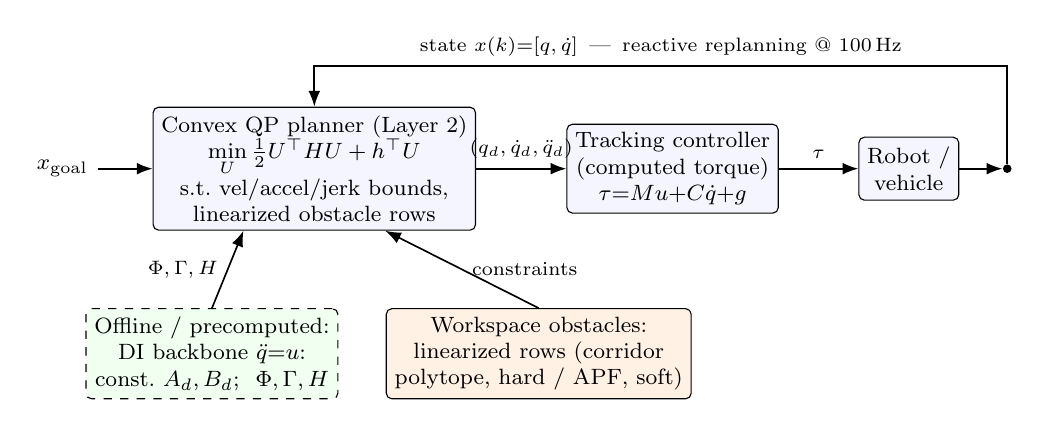
\begin{tikzpicture}[every node/.style={font=\footnotesize}]
  % ---- main execution row ----
  \node (goal) at (0,0) {$x_\text{goal}$};
  \node[blk] (qp) at (3.2,0) {Convex QP planner (Layer~2)\\ $\min\limits_{U}\frac12 U^\top H U+h^\top U$\\ s.t.\ vel/accel/jerk bounds,\\ linearized obstacle rows};
  \node[blk] (ctrl) at (7.75,0) {Tracking controller\\ (computed torque)\\ $\tau{=}Mu{+}C\dot q{+}g$};
  \node[blk] (plant) at (10.75,0) {Robot /\\ vehicle};
  \node[dot] (fb) at (12.0,0) {};
  % forward wires
  \draw[sig] (goal)--(qp);
  \draw[sig] (qp)-- node[above,font=\scriptsize]{$(q_d,\dot q_d,\ddot q_d)$} (ctrl);
  \draw[sig] (ctrl)-- node[above,font=\scriptsize]{$\tau$} (plant);
  \draw[sig] (plant)--(fb);
  % state feedback (reactive replanning)
  \draw[sig] (fb) |- ++(0,1.3) -| node[near start,above,font=\scriptsize]{state $x(k){=}[q,\dot q]$ \,---\, reactive replanning @ 100\,Hz} (qp.north);
  % ---- offline-precompute feeder ----
  \node[offb] (off) at (1.9,-2.35) {Offline / precomputed:\\ DI backbone $\ddot q{=}u$:\\ const.\ $A_d,B_d$;\ \ $\Phi,\Gamma,H$};
  \draw[sig] (off.north) -- node[left,font=\scriptsize,pos=0.5]{$\Phi,\Gamma,H$} ([xshift=-9mm]qp.south);
  % ---- obstacle / perception feeder ----
  \node[det] (obs) at (6.05,-2.35) {Workspace obstacles:\\ linearized rows (corridor\\ polytope, hard / APF, soft)};
  \draw[sig] (obs.north) -- node[right,font=\scriptsize,pos=0.5]{constraints} ([xshift=9mm]qp.south);
\end{tikzpicture}
\caption{Reactive predictive motion-planning architecture. The planner runs on
a virtual \emph{double-integrator backbone} ($\ddot q=u$), whose nilpotent
dynamics give a configuration-independent constant $A_d$, so the horizon
prediction matrices $\Phi,\Gamma$ and the QP Hessian $H$ are precomputed
\emph{offline} (left, dashed). Online, a convex QP (Layer~2) optimizes the
acceleration profile $U$ subject to velocity/acceleration/jerk bounds and
linearized workspace-obstacle rows (convex corridor polytope, hard; or APF goal
deflection, soft), emitting a time-indexed trajectory $(q_d,\dot q_d,\ddot q_d)$
to a downstream tracking controller and plant. Current state $x(k)$ and updated
obstacles re-enter every cycle, giving fixed-size reactive updates without
the stop-and-rebuild of path-first pipelines; Section~VI reports the measured
100\,Hz timing distribution and tail.}
\label{fig:arch}
\end{figure*}

Let \(q\in\mathbb{R}^n\) denote robot configuration and
\(p=f(q)\) task position. The planner generates
\((q(t),\dot q(t),\ddot q(t))\) satisfying waypoint, joint, velocity,
acceleration, and obstacle constraints; actuator commands are left to a
downstream tracking controller. The trajectory space is parameterized by
a virtual double-integrator backbone,
\begin{equation}
\label{eq:di-backbone}
  \ddot q = u,\qquad
  x=\begin{bmatrix}q^\top&\dot q^\top\end{bmatrix}^\top ,
\end{equation}
whose state contains planned positions and velocities. It is a configuration-independent
trajectory generator that makes acceleration a decision variable and
therefore keeps velocity and acceleration bounds linear.

\subsection{Double-Integrator Backbone from Dynamic
Cancellation}\label{a.-double-integrator-backbone-from-dynamic-cancellation}

The same backbone can also be derived from the standard manipulator
dynamics \(M(q)\ddot q+C(q,\dot q)\dot q+g(q)=\tau\). With the
computed-torque (inverse-dynamics) feedforward law---the same
cancellation used in the pHRI architecture of \cite{phri}---
\begin{equation}
\label{eq:computed-torque}
  \tau = M(q)u + C(q,\dot q)\dot q + g(q),
\end{equation}
substitution gives the backbone in \eqref{eq:di-backbone}, and hence
\begin{equation}
\label{eq:residual-dynamics}
\dot x = \begin{bmatrix} 0&I\\ 0&0 \end{bmatrix}x +
\begin{bmatrix} 0\\ I \end{bmatrix}u .
\end{equation}
The present work uses this residual model as a planning backbone rather
than as an impedance-regulation controller.

\subsection{Exact ZOH Discretization and the Constant A\_d Property}\label{b.-exact-zoh-discretization-and-the-constant-a_d-property}

Because the continuous system matrix is nilpotent, \(A_c^2=0\), exact
ZOH discretization over \(\Delta t\) gives
\begin{equation}
\label{eq:zoh}
A_d = \begin{bmatrix} 1 & \Delta t \\ 0 & 1 \end{bmatrix}, \qquad
B_d = \begin{bmatrix} \frac{\Delta t^2}{2} \\ \Delta t \end{bmatrix}.
\end{equation}
Unlike a physical plant linearization, this \(A_d\) is independent of
configuration, operating point, and joint index. Therefore the horizon
prediction matrices
\begin{equation}
\label{eq:prediction-matrices}
\Phi = \begin{bmatrix} A_d \\ A_d^2 \\ \vdots \\ A_d^N \end{bmatrix}, \qquad
\Gamma = \begin{bmatrix}
B_d & 0 & \cdots & 0 \\
A_d B_d & B_d & \cdots & 0 \\
\vdots & & \ddots & \vdots \\
A_d^{N-1} B_d & \cdots & A_d B_d & B_d
\end{bmatrix}
\end{equation}
are precomputed once and reused at every planning cycle. Online rollout
then reduces to
\begin{equation}
\label{eq:rollout}
X=\Phi x(k)+\Gamma U,
\end{equation}
decoupling prediction cost from robot configuration.

\section{Receding-Horizon Optimization}\label{iii.-receding-horizon-optimization-layer-2-qp-planner}

\subsection{Optimization Problem
Structure}\label{a.-optimization-problem-structure}

At each planning time step, the planner solves for the optimal
acceleration profile sequence across the prediction horizon:
\begin{equation}
\label{eq:decision-vector}
U = \begin{bmatrix} u^\top(0) & u^\top(1) & \cdots & u^\top(N-1) \end{bmatrix}^\top
\in \mathbb{R}^{nN}.
\end{equation}
where \(n\) is the number of joints and \(N\) is the horizon length
(e.g., \(nN = 7\times 20 = 140\) decision variables for the 7-DOF FR3
with \(N=20\)). The predicted trajectory follows \eqref{eq:rollout},
which is affine in \(U\); therefore kinematic bounds and linearized
obstacle rows remain convex. Absent obstacle coupling, the Hessian is
block-diagonal and the problem separates into \(n\) independent
per-joint QPs of size \(N\).

\subsection{Cost Function: Tracking and
Smoothness}\label{b.-cost-function-tracking-and-smoothness}

The objective function minimizes the weighted sum of tracking deviations
from a goal state \(x_{\text{goal}} = [q_{\text{goal}}, 0]^\top\) and
control effort. We write the stage cost with the conventional
\(\tfrac{1}{2}\) scaling,
\begin{align}
\label{eq:tracking-cost}
J(U)
&=\frac{1}{2}
\left(\Phi x(k)+\Gamma U-\mathbf{1}_N\otimes x_{\text{goal}}\right)^\top
\bar Q \nonumber\\
&\quad \times
\left(\Phi x(k)+\Gamma U-\mathbf{1}_N\otimes x_{\text{goal}}\right)
+\frac{1}{2}U^\top\bar R U .
\end{align}
so that collecting the terms depending on \(U\) gives
\begin{equation}
\label{eq:qp-objective}
\min_{U} \; \frac{1}{2} U^\top H U + h^\top U
\end{equation}
where:
\begin{equation}
\label{eq:qp-hessian-gradient}
H = \Gamma^\top \bar{Q} \Gamma + \bar{R}, \qquad
h = \Gamma^\top \bar{Q} \, x_{\text{free,err}}
\end{equation}
and
\(x_{\text{free,err}} = \Phi x(k) - \mathbf{1}_N \otimes x_{\text{goal}}\)
is the unforced deviation from the goal; \(h\) is the gradient at \(U=0\),
i.e.\ the linear-cost vector passed to OSQP. The remaining definitions
are: the full goal state \(x_{\text{goal}}=[q_{\text{goal}},0]^\top\)
replicated across all \(N\) horizon steps; stage weights
\(Q = \text{blkdiag}(K_q, D_q)\) on position/velocity error; control cost
\(R\) regularizing acceleration; terminal weight \(Q_f = \gamma Q\)
(\(\gamma \approx 5\)--\(10\)); and horizon-stacked
\(\bar Q = \mathrm{blkdiag}(Q,\dots,Q,Q_f)\), \(\bar R = I_N \otimes R\).

Because \(H\) is the sum of a positive semi-definite matrix (from
\(\bar{Q}\)) and a positive definite matrix (from \(\bar{R}\) with
\(R \succ 0\)), the QP is \textbf{strictly convex} for all
configurations and all time steps. A unique global minimizer exists and
is found efficiently by operator-splitting solvers such as OSQP \cite{osqp}
with warm-starting, converging in under 0.5 ms for the decoupled
box-constrained QP and in a few milliseconds for the coupled-obstacle QP
(Section~\ref{b.-fr3-manipulator-results}).

\textbf{Weight tuning guidance.} The weights have intuitive roles:
\(K_q\) sets convergence aggressiveness (larger pulls to the goal faster
but risks acceleration saturation); \(D_q\) provides damping, with
\(D_q \approx 2\sqrt{K_q}\) giving a critically-damped response; \(R\)
trades smoothness against speed; and the terminal multiplier
\(\gamma = 5\)--\(10\) compensates for the finite horizon at
\(N \geq 20\). The weights are per-joint scalars, tuned by increasing
\(K_q\) until goals are reached within limits, then \(D_q\) until overshoot
disappears, then \(R\) if jerk is excessive. The experiments do not share a
single setting, so we list what each actually uses: the static FR3 benchmark
and the Hessian-norm study run the planner defaults \(K_q=50\), \(D_q=0\),
\(R=0.05\,I\), \(\gamma=8\); the FR3 dynamic-obstacle study uses
\(K_q=6\), \(D_q=8\), \(R=0.05\,I\), \(\gamma=8\); the Cartesian-DI vehicle
benchmark uses \(K_q=12\), \(D_q=4\), \(R=0.3\,I\), \(\gamma=6\); and the
jerk-bounded lateral planner reported in Table~\ref{tab:av-steering} uses
\(w_q=20\), \(w_a=0.2\), \(w_r=0.02\), \(\gamma=10\). Note that
\(D_q=0\) in the static FR3 case: there the terminal multiplier and the
acceleration bound alone suppress overshoot, so no velocity-error damping is
needed, and the \(D_q\approx2\sqrt{K_q}\) guidance above applies to the
cases that do use it rather than to every experiment reported here.

\subsection{Kinematic Hard
Constraints}\label{c.-kinematic-hard-constraints}

Physical joint limits are enforced as hard inequality constraints on the
predicted state and input sequences. For each joint \(i\) and each step
\(k\) along the horizon:
\begin{align}
\label{eq:kinematic-bounds}
-\dot{q}_{i,\max} &\leq \dot{q}_{i}(k) \leq \dot{q}_{i,\max},
&& k=1,\dots,N, \nonumber\\
-u_{i,\max} &\leq u_i(k) \leq u_{i,\max},
&& k=0,\dots,N-1 .
\end{align}

Since the predicted states are affine in \(U\) by \eqref{eq:rollout},
the bounds in \eqref{eq:kinematic-bounds} translate to linear inequalities
\(C_{\text{kin}} U \leq d_{\text{kin}}\) assembled once from the
precomputed \(\Gamma\) matrix and fixed online. Optionally, joint
position limits \(q_{i,\min} \leq q_i(k) \leq q_{i,\max}\) can be
appended with no additional computational overhead.

Because the velocity bounds are imposed without slack, feasibility of the
QP assumes the current state lies inside the velocity polytope; if a
disturbance drives \(\dot q(k)\) outside it, the box rows should be
softened on the first horizon step or a terminal maximal-braking-to-rest
set appended to recover recursive feasibility (see
Section~\ref{scope-and-limitations}).

\section{Incorporating Workspace Obstacle
Avoidance}\label{iv.-incorporating-workspace-obstacle-avoidance}

The linearity of the predicted joint positions with respect to \(U\)
makes it straightforward to incorporate obstacle avoidance constraints
without breaking convexity. Two complementary methods are presented.

\subsection{Convex Corridor Polytope Constraints (Hard
Constraints)}\label{a.-convex-corridor-polytope-constraints-hard-constraints}

Cartesian obstacles detected by perception systems are represented as
half-space inequalities in task space:
\begin{equation}
\label{eq:workspace-halfspace}
A_{\text{obs}} \, p(k) \leq b_{\text{obs}}
\end{equation}
where \(p(k) \in \mathbb{R}^3\) is the predicted end-effector (or link)
position at step \(k\). Using the robot's forward kinematics linearized
at the current operating point via the translational Jacobian
\(J_v(q_0)\):
\begin{equation}
\label{eq:fk-linearization}
p(k) \approx p_0 + J_v(q_0)\bigl(q(k) - q_0\bigr)
\end{equation}
the workspace constraint in \eqref{eq:workspace-halfspace} becomes:
\begin{equation}
\label{eq:workspace-linear-row}
A_{\text{obs}} J_v(q_0) \, \Delta q(k)
\leq b_{\text{obs}} - A_{\text{obs}} p_0
\end{equation}
where \(\Delta q(k) = q(k) - q_0\) is linear in \(U\) through
\(\Gamma\). To make the QP row explicit, let
\(E_{q,k}\in\mathbb{R}^{n\times 2nN}\) be the selector that extracts the
\(n\)-dimensional joint-position block of the stacked state \(X\) at
horizon step \(k\) (a row of \(n\times n\) identity blocks, zero
elsewhere), so
\begin{equation}
\label{eq:position-selector}
q(k)=E_{q,k}\bigl(\Phi x(k_0)+\Gamma U\bigr).
\end{equation}
Define \(C_{\text{obs},k}=A_{\text{obs}}J_v(q_0)E_{q,k}\Gamma\). Then
each obstacle row has the affine form
\begin{equation}
\label{eq:obstacle-row}
\begin{aligned}
 C_{\text{obs},k}U
&\le b_{\text{obs}}-A_{\text{obs}}p_0 \\
&\quad
-A_{\text{obs}}J_v(q_0)\bigl(E_{q,k}\Phi x(k_0)-q_0\bigr)
=: d_{\text{obs},k}.
\end{aligned}
\end{equation}
Thus the free-response term is absorbed into the right-hand side, and
the obstacle constraint becomes a set of affine inequalities in \(U\),
fully compatible with the convex QP structure.

\textbf{Approximation quality.} Because \(J_v(q_0)\) is held constant over
the horizon, these rows are a first-order local approximation of the safe
corridor---exact near \(q_0\), increasingly inaccurate away from it, and
not automatically conservative. Re-linearizing every cycle refreshes it; a
conservative half-space additionally tightens each row by a bound on the
linearization error. From the second-order Taylor remainder, with
\(H_p(q_0)\) the position Hessian, the true end-effector position
satisfies
\begin{equation}
\label{eq:linearization-error}
\|p(q) - (p_0 + J_v(q_0)\Delta q)\|
\leq \tfrac{1}{2} \|H_p(q_0)\|_F \|\Delta q\|^2
\end{equation}
where \(\|\cdot\|_F\) is the Frobenius norm. For an obstacle half-space
row \(a^\top p\le b\), a conservative tightened row is
\begin{equation}
\label{eq:tightened-row}
a^\top\bigl(p_0+J_v(q_0)\Delta q(k)\bigr)
\le b-\|a\|\,\varepsilon_p,
\end{equation}
with
\(\varepsilon_p \geq \tfrac{1}{2}\|H_p\|_{F}\|\Delta q\|^2\) from
\eqref{eq:linearization-error}. For the FR3, \(\|H_p\|_F\) sampled at 5000
joint-range configurations has mean \(1.64\) and 95th-percentile \(1.96\)
m/rad² (\texttt{fr3\_hessian\_norm.py}). The measured end-horizon error
grows quadratically with joint-speed$\times$horizon (harness: 7.1 mm at
25\% speed over 0.1 s, 106.4 mm at 50\% over 0.2 s, 1.03 m at full speed
over 0.4 s). The Frobenius bound is a worst case over directions and is
therefore loose: at 50\% speed over the \(N=20\) horizon
\(\|\Delta q\|_2\approx 1.0\) rad, so \eqref{eq:tightened-row} prescribes
\(\varepsilon_p \gtrsim \tfrac{1}{2}(1.96)(1.0)^2 \approx 1.0\) m, whereas
the realized end-horizon drift is only 106 mm because the executed motion
does not excite the worst-case curvature. In practice the margin should
therefore be set from the \emph{measured} drift---a workspace percentile of
the end-horizon error---rather than from the conservative Frobenius bound,
and the horizon shortened for fast motions; at modest speeds a
centimetre-scale margin suffices.

\textbf{Accuracy of the constraint guarantee.} The QP guarantees
satisfaction of the \emph{linearized} safe-corridor constraints: no
predicted trajectory penetrates the declared linearized obstacle polytope.
A true nonlinear collision-clearance guarantee additionally requires
conservative tightening by \(\varepsilon_p\), nonlinear collision checking
of the accepted rollout, or both; for non-convex environments, standard
safe-corridor decomposition \cite{safe_corridor} can be applied upstream.

\textbf{Multiple obstacles.} Method A appends \(M\) independent half-space
sets, keeping convexity at mildly increasing solver cost; if rows conflict
the QP becomes infeasible, resolved by per-obstacle slacks \(s_m \geq 0\)
with penalty \(\mu \|s\|^2\). Method B sums individual APF repulsion
fields, avoiding infeasibility but inheriting the local-minimum risk of
scalar APF methods.

\subsection{Artificial Potential Field Target Deflection (Soft
Constraint)}\label{b.-artificial-potential-field-target-deflection-soft-constraint}

For scenarios requiring maximum solver throughput, an alternative
soft-constraint approach using Artificial Potential Fields (APF) \cite{khatib1986}
is available. An obstacle at position \(p_{\text{obs}}\) with influence
radius \(\rho_0\) and repulsive gain \(\eta\) generates a task-space
repulsive potential:
\begin{equation}
\label{eq:apf-potential}
\mathcal{U}_{\text{rep}}(p) =
\begin{cases}
\frac{1}{2} \eta
\left(\frac{1}{\|p - p_{\text{obs}}\|} - \frac{1}{\rho_0}\right)^2,
& \|p - p_{\text{obs}}\| \leq \rho_0,\\
0, & \text{otherwise}.
\end{cases}
\end{equation}
The negative gradient
\(g_{\text{rep}}(p)=-\nabla \mathcal{U}_{\text{rep}}(p)\), treated as a
synthetic direction field rather than a physical force, is normalized as
\(\hat{g}_{\text{rep}}=g_{\text{rep}}/(\|g_{\text{rep}}\|+\epsilon)\) and
mapped to a heuristic joint-space target shift via the Jacobian
pseudo-inverse,
\begin{equation}
\label{eq:apf-target-shift}
\delta q_{\text{obs}} = K \, J_v^+(q) \, \hat{g}_{\text{rep}},
\end{equation}
where the scalar gain \(K > 0\) absorbs all dimensional scaling. (In the
simulations below the same idea is implemented as a velocity/reference
deflection with an optional tangential component to avoid stalls; in both
cases APF changes the reference rather than adding a hard row.) The target
fed to the cost function is then updated online:
\begin{equation}
\label{eq:apf-target}
q_{\text{target}}(k) = q_{\text{goal}} + \delta q_{\text{obs}} .
\end{equation}
This bypasses inequality rows entirely, preserving the minimal QP
structure and maximizing solve speed. The trade-off is that obstacle
avoidance is enforced softly through the cost function rather than
guaranteed through hard constraints; APF-based avoidance is also
susceptible to local minima in complex environments (see Section VIII).

\textbf{Local minima mitigation.} When the APF gradient vanishes the
planner stalls; three escape strategies are available: (1) \emph{waypoint
injection}---insert a lateral waypoint after a no-progress timeout
(e.g.\ 0.5 s); (2) \emph{random perturbation}---add a small random shift to
\(q_\text{target}\) for a few cycles; (3) \emph{hybrid switch}---activate
the Method-A hard polytope (with slack) on stall. Option (1) is preferred
as it adds no solver overhead. The two methods are complementary: hard
polytope constraints for static infrastructure, APF deflection for dynamic
obstacles.

\section{Architectural Properties}\label{v.-architectural-properties}

\subsection{Constant-Structure MPC and Fixed-Size Replanning
Updates}\label{a.-constant-structure-mpc-and-bounded-replanning-latency}

The central property is that all dynamics prediction matrices (\(\Phi\),
\(\Gamma\), \(H\)) are precomputed offline and never rebuilt online;
obstacle rows are re-assembled each cycle but still project \(J_v\) through
the fixed \(\Gamma\). Each cycle thus executes a QP whose dynamics structure
is fixed at initialization. Per-cycle work consists of one QP update and
solve for a given active set---growing with the obstacle-row count but
independent of configuration and free of prediction-matrix rebuilds. This is distinct
from configuration-dependent MPC (which recomputes prediction matrices at
each linearization point) and from batch planning (TOTG, TOPP-RA, where any
workspace change triggers a full rebuild). The constant-\(A_d\) property makes
the update size predictable; it does not by itself establish a hard execution-time
bound, so Section~VI reports p95 and maximum latency separately.

\subsection{Elimination of Spatial-to-Temporal
Transformations}\label{b.-elimination-of-spatial-to-temporal-transformations}

Traditional pipelines solve a separate time-parameterization problem---given
a path \(\sigma(s)\), find \(s(t)\) satisfying velocity/acceleration
limits---decoupled from obstacle avoidance and re-executed whenever the path
changes. The proposed framework has no geometric path: positions,
velocities, and accelerations along the horizon are generated simultaneously
in one QP, so the \(s \leftrightarrow t\) conversion stage and its
singularities (Section VI.A) are eliminated by construction.

\subsection{\texorpdfstring{\(C^1\) Output with Hard-Bounded
Acceleration}{C. C\^{}1 Output with Hard-Bounded Acceleration}}\label{c.-c1-output-with-hard-bounded-acceleration}
Because the proposed planner uses joint acceleration \(u_i\) as the
direct optimization variable and enforces acceleration bounds as hard
constraints, the output \((q_d, \dot{q}_d)\) is \(C^1\) with
\(\ddot{q}_d\) hard-bounded at all times. Since \(u_i\) is held over
each control cycle (zero-order hold), \(\ddot{q}_d\) is
piecewise-constant and steps between cycles; full \(C^2\) continuity
requires jerk to be included as the optimization variable within a
higher-order planning backbone.

\subsection{Piecewise-Jerk Triple-Integrator Extension}\label{d.-piecewise-jerk-triple-integrator-extension-for-continuous-acceleration}

When continuous acceleration is required---to reduce torque-rate
excitation, satisfy comfort limits, or bound steering-rate in vehicle
applications---the same constant-\(A_d\) principle extends to a
triple-integrator backbone that optimizes jerk \(\dddot q_i = j_i\) on the
state \(z_i=[q_i,\dot q_i,\ddot q_i]^\top\). The continuous system matrix
is again nilpotent (\(A_c^3=0\)), so exact ZOH discretization gives the
configuration-independent
\begin{equation}
\label{eq:triple-zoh}
A_d^{(3)} =
\begin{bmatrix}
1&\Delta t&\tfrac{1}{2}\Delta t^2\\
0&1&\Delta t\\
0&0&1
\end{bmatrix},
\qquad
B_d^{(3)} =
\begin{bmatrix}
\tfrac{1}{6}\Delta t^3\\
\tfrac{1}{2}\Delta t^2\\
\Delta t
\end{bmatrix}.
\end{equation}
so the prediction matrices remain precomputable offline. With jerk held
constant per interval, \(\ddot q(t+\tau)=\ddot q(t)+\tau j(t)\) keeps
acceleration continuous across samples while jerk is piecewise-constant,
raising output smoothness from \(C^1\) to \(C^2\) (\(q_d\in C^2\),
\(\dot q_d\in C^1\), \(\ddot q_d\in C^0\)) with hard linear bounds now
available on velocity, acceleration, and jerk.

The trade-off is a larger state and extra predicted-state rows, though the
decision sequence is still length \(nN\), now a jerk sequence
\(J=[j(0),\dots,j(N-1)]\) rather than acceleration. The AV steering-rate
benchmark (§VI.C) uses exactly this for the lateral channel, since steering
rate depends on lateral jerk.

Its objective differs from \eqref{eq:tracking-cost} and is stated here
explicitly. Writing \(\Gamma_p,\Gamma_a\) for the position and acceleration
blocks of the triple-integrator prediction matrices, \(e_p=\Phi_p z-y_{\rm
goal}\) for the free-response lateral offset error and \(a_{\rm free}=\Phi_a z\)
for the free-response lateral acceleration, the lateral planner minimizes
\begin{align}
\label{eq:lateral-cost}
J(U)&=\tfrac12\left(\Gamma_pU+e_p\right)^\top \bar W_q\left(\Gamma_pU+e_p\right)
\nonumber\\
&\quad+\tfrac12 w_a\left\|\Gamma_aU+a_{\rm free}\right\|^2
+\tfrac12 w_r\|U\|^2 ,
\end{align}
with \(\bar W_q=\mathrm{diag}(w_q,\dots,w_q,\gamma w_q)\) and
\(w_q=20\), \(w_a=0.2\), \(w_r=0.02\), \(\gamma=10\). Two differences from
\eqref{eq:tracking-cost} matter: the middle term penalizes the predicted
\emph{absolute} lateral acceleration rather than a velocity error, because
lateral acceleration is the comfort-relevant quantity here; and there is no
velocity-error term at all, since the lateral channel tracks an offset rather
than a velocity profile. Velocity, acceleration, and jerk remain hard rows in
the constraint set. The jerk row bounds lateral jerk, not steering
rate itself: because
\(\delta=\arctan\!\big(L(\dot x\ddot y-\dot y\ddot x)/(\dot x^2+\dot y^2)^{3/2}\big)\)
depends nonlinearly on the lateral velocity and acceleration as well, a given
\(j_{\max}\) implies a steering-rate cap only once those terms are accounted
for at the operating point. The harness therefore \emph{measures} the
resulting steering rate (§VI.C) rather than constraining it in the QP.

The rest of the paper uses the double-integrator backbone as the main
manipulator planner because it is the smallest model that enforces
velocity and acceleration limits directly and gives the fastest QP. The
triple-integrator form is a drop-in extension when continuous
acceleration or explicit jerk bounds are application-critical.

\subsection{Analytical LQR Characterization of the Double-Integrator
Backbone}\label{e.-analytical-lqr-characterization-of-the-double-integrator-backbone}

As background, the unconstrained infinite-horizon limit of the planner is
the standard LQR law \(u=u_{ff}-K(x-x_r)\), \(K=R^{-1}B^\top P\), with
\(P\) solving the Algebraic Riccati Equation
\(A^\top P+PA-PBR^{-1}B^\top P+Q=0\) (\(u_{ff}=\ddot q_r\), zero for fixed-goal
regulation). This situates the method within standard optimal control and
relates the weights to the closed-loop second-order behavior. The
constrained planner is the finite-horizon counterpart: the same backbone
solved as a receding-horizon QP enforcing velocity, acceleration, joint,
and obstacle constraints---mathematically close to linear MPC
\cite{mayne2000}, but on a virtual trajectory state rather than a plant
linearization. The robot model enters through kinematics and workspace
constraints \cite{khatib1987}; the output is the reference trajectory
\(\mathcal T=\{q_d,\dot q_d,\ddot q_d\}\) for a downstream controller.

\section{Experimental Evaluation}\label{vi.-experimental-evaluation}

We evaluate the proposed planner against a path-first Time-Optimal
Trajectory Generation pipeline on a 7-DOF Franka FR3 manipulator and on
an autonomous-vehicle steering task. Both planners receive identical
waypoints and kinematic limits and emit \((q_d, \dot q_d, \ddot q_d)\)
sampled at the same \(\Delta t\); all numbers reported below are
measured by the accompanying open harness: the scripts in
\texttt{benchmarks/}, which print each reported table to stdout, with the
rendered figures and the AV trajectory export collected in
\texttt{simulationResults/}. Because several benchmark modules re-export a
shared planner from a sibling repository, a frozen snapshot with those modules
inlined is shipped as \texttt{benchmarks\_standalone.zip}, together with source
provenance and a dependency manifest. All non-MuJoCo tables reproduce from that
archive alone. The computed-torque execution table additionally requires the
third-party Franka model/assets via \texttt{FR3\_XML}; those assets are not
bundled. Raw per-trial dumps are not committed---the harness recomputes
them---and wall-clock values are hardware/OS dependent, so deterministic
constraint and geometry metrics are distinguished from timed measurements. The
TOTG reference uses the numerical-integration TOPP core---circular-blend
path (Kunz--Stilman geometry \cite{kunz2012}), time-optimal forward/backward
sweep on \(\dot s^2\) \cite{toppra}, then \(s\!\to\!t\) inversion and
resampling.

\textbf{Scope of comparison.} We compare against the path-first family
(TOTG, TOPP-RA), a resolved-rate-plus-APF baseline, and a sampling-based
MPPI baseline on the planar dynamic-obstacle test
(Section~\ref{d.-bounded-latency-reactive-replanning}). Online nonlinear MPC
and CHOMP/TrajOpt are deferred to future work; the present planner's appeal
is the constant-\(A_d\) precomputation and fixed-size online update, while
richer nonlinear formulations address a broader planning model.

This section reports four evaluation axes: reactive latency, jerk/
smoothness, constraint fidelity, and the execution-time gap. On static
paths, time-optimal path parameterization is faster; the fixed time-domain
QP trades a small amount of that global time optimality for fixed-size reactive
updates, explicit limit satisfaction, and smoother command profiles.

\subsection{\texorpdfstring{Path-First \(t\!\leftrightarrow\!s\)
Conversion Artifacts}{Path-First t-s Conversion Artifacts}}\label{a.-path-first-tleftrightarrows-conversion-artifacts}

The \(s\!\to\!t\) reconstruction differentiates the geometric path,
\[\eqfit{\ddot q(t) = q'(s)\,\ddot s \;+\; \underbrace{q''(s)}_{\text{curvature vector}}\,\dot s^2 .}\]
Two pathologies follow from the standard circular-blend path
representation. First, \(q''(s)\) jumps at every blend seam (\(0\) on a
straight segment, \(1/r\) on a circular arc), so the reconstructed
\(\ddot q\) is discontinuous, with the jump scaling as \(\dot s^2\).
Second, \(t(s)=\int ds/\dot s\) is singular wherever \(\dot s \to 0\)
(rest points, tight near-reversal blends), making the uniform-time
resample ill-conditioned. These artifacts are a property of the
circular-blend path representation, not of time parameterization per se.
Replacing circular blends with a \(C^2\) path (e.g., cubic splines)
removes them, as confirmed below. The time-first planner never forms
\(s\); its \(\ddot q\) is the bounded decision variable, so neither
pathology can arise.

The \((s,\dot s)\) phase plane (Fig.~\ref{fig:topp-phaseplane}) makes the singularity visible:
the maximum-velocity curve and optimal profile \(\dot s^*(s)\) dip
toward zero at the tight blend---severely on the near-reversal, where
\(\dot s\to0\) drives \(t(s)\) singular.

\begin{figure}[t]
\centering
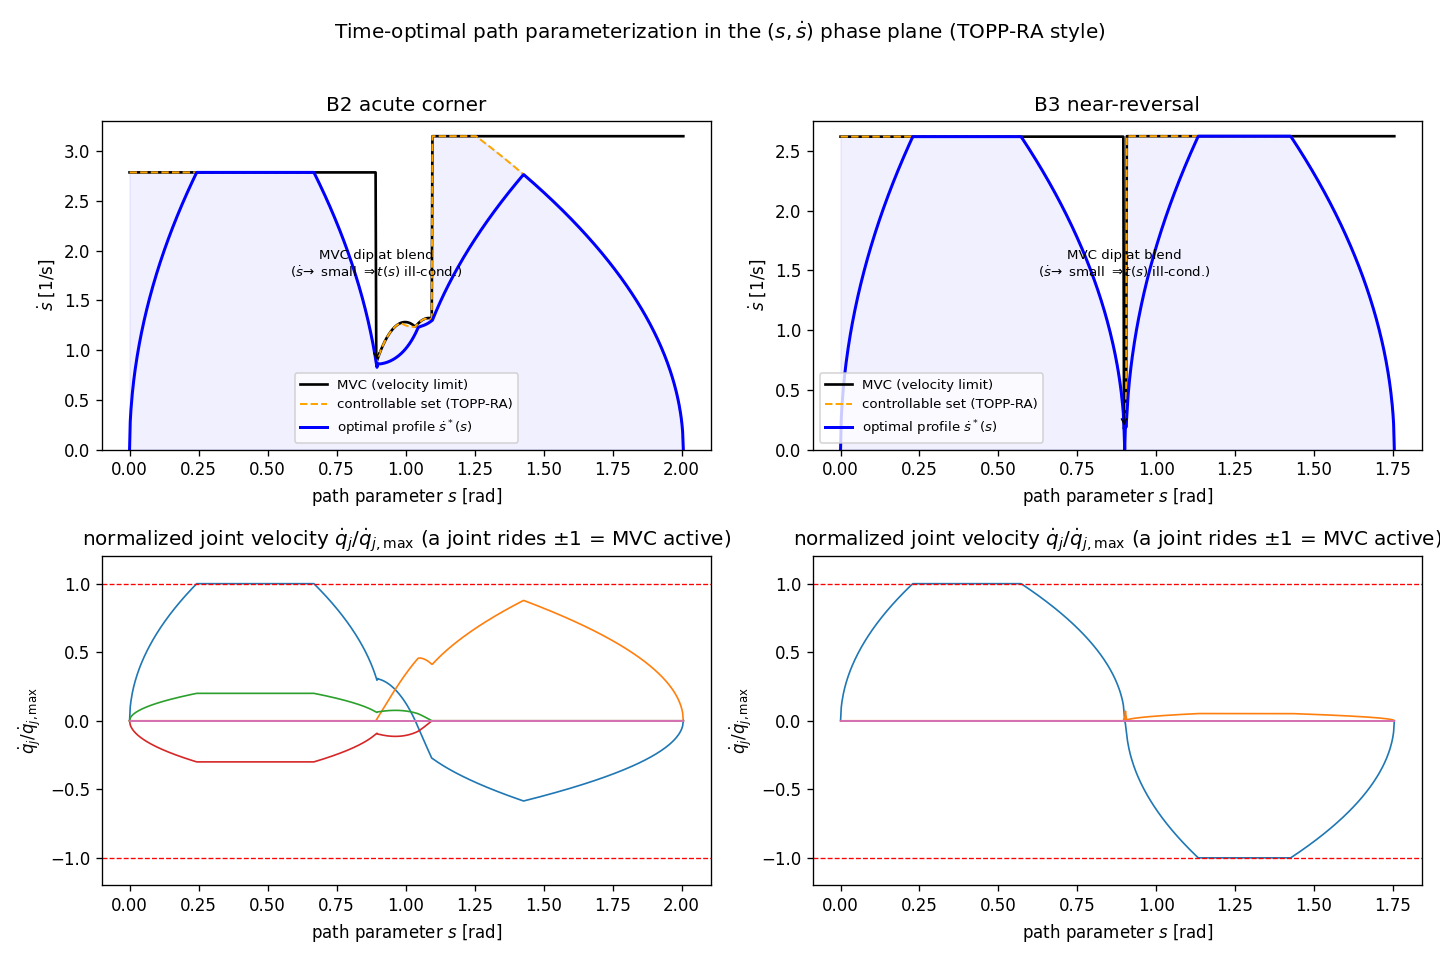
\includegraphics[width=\linewidth]{simulationResults/topp_phaseplane.png}
\caption{Time-optimal path parameterization in the
\((s,\dot s)\) phase plane (TOPP-RA style). The optimal profile dips at
the tight blend and---on the near-reversal---plunges to
\(\dot s\approx 0\), exactly where the \(s\!\to\!t\) map becomes
singular.}
\label{fig:topp-phaseplane}
\end{figure}

\subsection{FR3 Manipulator
Results}\label{b.-fr3-manipulator-results}

Stresses are concentrated in two joints for interpretability while all
seven are planned. The decisive metric is the peak acceleration ratio
\(\lVert\ddot q\rVert_\infty/\ddot q_{\max}\): a value above \(1\) means
the emitted trajectory violates the declared acceleration limit. The DI
planner enforces this as a hard QP constraint and is pinned at \(1.000\)
with zero violations in every scenario.

{% converted Pandoc table
\begin{table*}[t]
\caption{FR3 Manipulator Benchmark Results}
\label{tab:fr3-main-results}
\centering
\footnotesize
\setlength{\tabcolsep}{3pt}
\begin{tabular}{@{}
  >{\raggedright\arraybackslash}p{(\linewidth - 14\tabcolsep) * \real{0.1250}}
  >{\raggedright\arraybackslash}p{(\linewidth - 14\tabcolsep) * \real{0.1250}}
  >{\raggedright\arraybackslash}p{(\linewidth - 14\tabcolsep) * \real{0.1250}}
  >{\raggedright\arraybackslash}p{(\linewidth - 14\tabcolsep) * \real{0.1250}}
  >{\raggedright\arraybackslash}p{(\linewidth - 14\tabcolsep) * \real{0.1250}}
  >{\raggedright\arraybackslash}p{(\linewidth - 14\tabcolsep) * \real{0.1250}}
  >{\raggedright\arraybackslash}p{(\linewidth - 14\tabcolsep) * \real{0.1250}}
  >{\raggedright\arraybackslash}p{(\linewidth - 14\tabcolsep) * \real{0.1250}}@{}}
\toprule\noalign{}
\begin{minipage}[b]{\linewidth}\raggedright
Scenario
\end{minipage} & \begin{minipage}[b]{\linewidth}\raggedright
DI \(T\) {[}s{]}
\end{minipage} & \begin{minipage}[b]{\linewidth}\raggedright
TOTG \(T\) {[}s{]}
\end{minipage} & \begin{minipage}[b]{\linewidth}\raggedright
DI accel ratio
\end{minipage} & \begin{minipage}[b]{\linewidth}\raggedright
TOTG accel ratio
\end{minipage} & \begin{minipage}[b]{\linewidth}\raggedright
TOTG accel viol.
\end{minipage} & \begin{minipage}[b]{\linewidth}\raggedright
DI jerk RMS
\end{minipage} & \begin{minipage}[b]{\linewidth}\raggedright
TOTG jerk RMS
\end{minipage} \\
\midrule\noalign{}
B1 point-to-point & 2.02 & \textbf{0.59} & 1.000 & 1.000 & 0 &
\textbf{22} & 143 \\
B2 acute corner (tight blend) & 1.92 & \textbf{1.23} & 1.000 &
\textbf{1.047} & 2 & 36 & 133 \\
B3 near-reversal & 1.99 & 1.07 & 1.000 & up to \textbf{3.13} & 0--1 & 29
& 166 \\
B4 dense (24 waypoints) & 13.24 & \textbf{3.83} & 1.000 & \textbf{1.445}
& 49 & \textbf{54} & 333 \\
\bottomrule\noalign{}
\end{tabular}
\end{table*}
}

Separating the decoupled and coupled cases, the single-threaded Python
harness (OSQP tolerance \(10^{-6}\), warm-started, fixed KKT sparsity on
the coupled update path) solves the 140-variable decoupled box-constrained
QP (7 DOF, \(N{=}20\)) in 0.03--0.08 ms mean on the current workstation.
Across three repeated fixed-sparsity runs, the 141-variable coupled obstacle
QP (Method A) has solve mean/p95/max ranges of
1.87--2.07/3.87--4.49/8.34--9.19 ms; including Python assembly and updates,
the full-cycle ranges are 4.74--5.07/6.60--7.70/12.26--18.48 ms.

A horizon sweep \(N=\{10,20,30,40\}\) on the same coupled FR3
dynamic-obstacle problem (\texttt{sweep\_N.py}) confirms why \(N=20\)
(0.2 s) is the default. Because the scenario uses a velocity-law/APF
reference, completion (1.83--1.86 s) and min EE clearance ($\approx$0.30 m)
are nearly insensitive to \(N\); the dominant trend is computational, with
coupled-QP solve p95 rising steeply from 1.0 ms (\(N{=}10\)) and 4.4 ms
(\(N{=}20\)) to 20.4 ms (\(N{=}30\)) and 55.6 ms (\(N{=}40\)). For pure
position-tracking waypoints \(N=10\) instead inflates time-to-goal, so
\(N=20\) balances both regimes.

\textbf{Comparison scope.} The acceleration violation metric compares
the trajectory as emitted by each planner---i.e., the command sequence
as-sent to the controller, with no downstream smoothing or
re-interpolation applied to either planner's output. In practice, some
systems apply a final spline pass to the TOTG output before execution,
which would reduce or eliminate the resampling-induced violations on B2
and B4; under such post-processing the DI planner's zero-violation
advantage on those scenarios shrinks. The advantage on B3 (near-reversal
singularity) and in the reactive scenarios (Sections VI.D--F) is
independent of downstream smoothing.

Figure~\ref{fig:fr3-accel-compare} plots the acceleration ratio over time
for each scenario: the DI curve never crosses \(1\), while the TOTG curve
spikes above it at blend seams.

\begin{figure}[t]
\centering
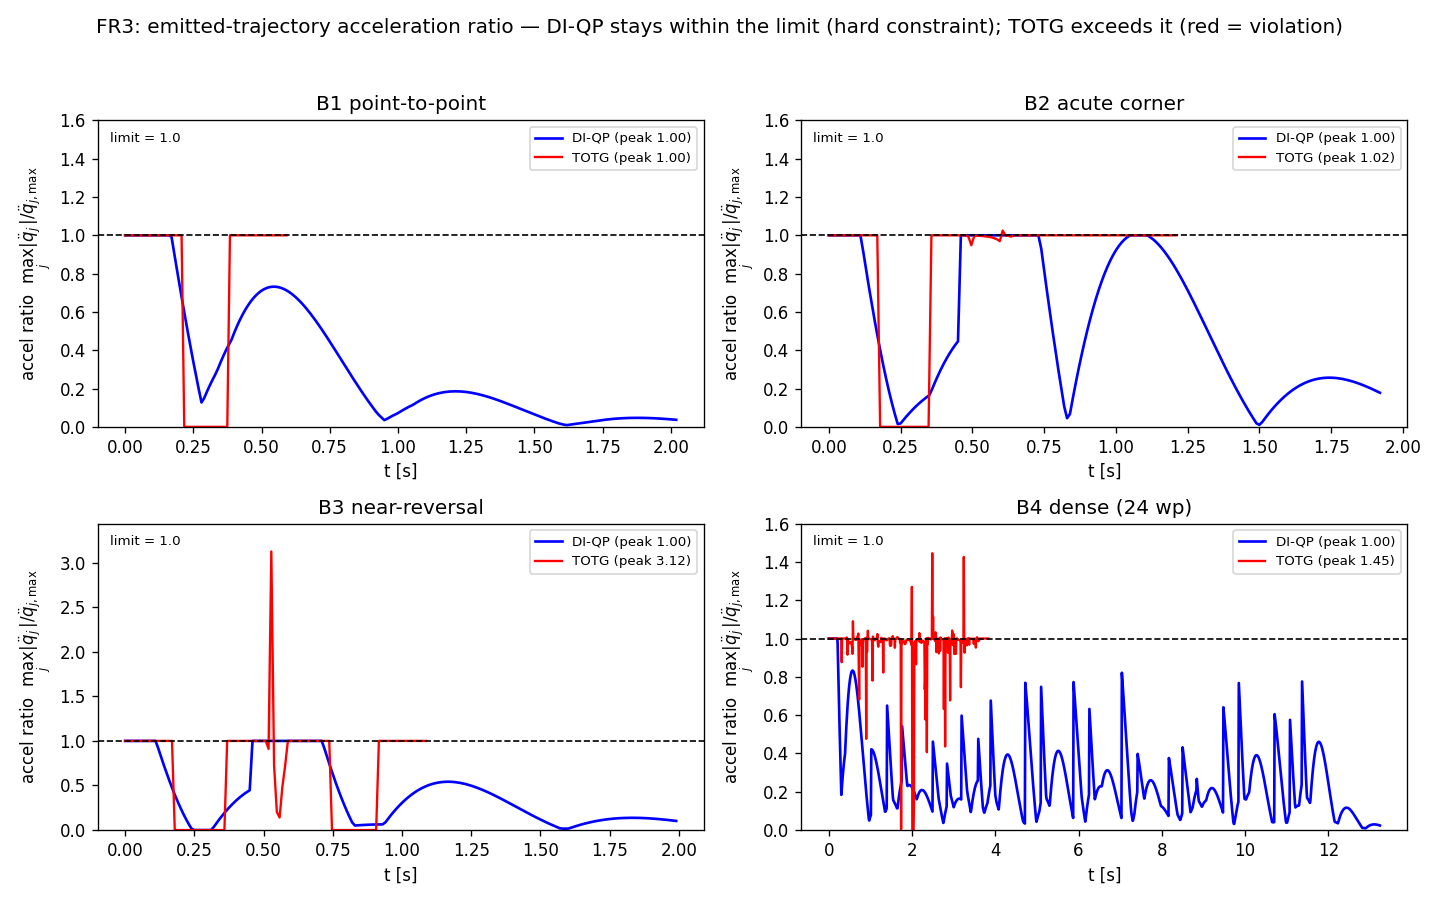
\includegraphics[width=\linewidth]{simulationResults/fr3_accel_compare.png}
\caption{FR3 emitted-trajectory acceleration ratio
\(\max_j|\ddot q_j|/\ddot q_{j,\max}\) over time, DI-QP (blue) vs TOTG
(red), B1--B4; dashed line is the limit. DI-QP is pinned within the limit
by hard constraints; TOTG exceeds it at blend seams (B2 \(1.047\times\),
B3 up to \(3.13\times\), B4 \(1.445\times\)). The B3 spike is
blend-dependent (drops to \(1.00\times\) under TOPP-RA/\(C^2\)); the
intrinsic path-first issues are the \(\dot s\to0\) singularity and
curvature-discontinuous reconstruction, not the spike magnitude.}
\label{fig:fr3-accel-compare}
\end{figure}

In \textbf{B3 (near-reversal)} the blend radius collapses,
\(\dot s\to 0\), and the parameterization becomes singular:
\(\max(1/\dot s)\to\infty\) and the \(s\!\to\!t\) conversion fails
(flagged and capped by the harness). In \textbf{B4} the path-first
command breaks the acceleration limit by 45\% at 49 samples. The DI
planner remains feasible and smooth throughout.

\textbf{Robustness to the parameterizer (TOPP-RA).} Re-running with
reachability-based \textbf{TOPP-RA} \cite{toppra}---designed to be robust
at dynamic singularities---the structural findings persist: the acute
corner still exceeds the acceleration limit (\(1.020\times\) vs
\(1.025\times\)), the dense path still violates (\(1.12\times\)), and the
near-reversal stays singular (\(\min\dot s = 0\)) for both parameterizers.
TOPP-RA softens magnitudes (the \(3.13\times\) B3 spike drops to
\(1.000\times\)), separating what is implementation-dependent (spike size)
from what is intrinsic to path-first (the violation from
curvature-discontinuous reconstruction and the \(\dot s\to0\) singularity).
Replacing circular blends with a \(C^2\) spline removes the B2/B4
violations entirely, so TOPP-RA on a \(C^2\) path matches the DI planner
on those metrics.

\textbf{Time-optimality.} TOTG is the lower bound by construction. With
the smooth quadratic-cost setting, the DI completion-time ratios are
\(3.4\times\) in B1 and \(3.5\times\) in B4. Supplying the analytic
time-optimal velocity-law reference (velocity-dominant weights,
\texttt{improve\_test.py}) recovers the gap to \(1.06\)--\(1.32\times\)
while the DI-QP still preserves zero limit violations, as quantified in
Table~\ref{tab:velocity-law}. The recovery trades
smoothness for speed, raising jerk RMS by roughly an order of magnitude:
the velocity-law reference is an explicit speed-versus-smoothness
selector. Thus the DI planner
remains feasible by construction with respect to the declared time-domain
bounds, while path-first feasibility can be lost after circular-blend
reconstruction and uniform-time resampling unless a smoother path
representation or downstream post-processing is used.

{% converted Pandoc table
\begin{table}[t]
\caption{Velocity-Law Recovery of the Time-Optimality Gap (FR3)}
\label{tab:velocity-law}
\centering
\footnotesize
\setlength{\tabcolsep}{4pt}
\begin{tabular}{@{}llrrr@{}}
\toprule\noalign{}
Scenario & Planner & \(T\) {[}s{]} & vs TOTG & Jerk RMS \\
\midrule\noalign{}
B1 & baseline DI    & 2.02 & \(3.42\times\) & \textbf{22.4} \\
B1 & velocity-law DI & 0.78 & \textbf{\(1.32\times\)} & 139.9 \\
B1 & TOTG            & 0.59 & \(1.00\times\) & 143.0 \\
\midrule
B2 & baseline DI    & 1.92 & \(1.59\times\) & \textbf{36.2} \\
B2 & velocity-law DI & 1.28 & \textbf{\(1.06\times\)} & 293.2 \\
B2 & TOTG            & 1.21 & \(1.00\times\) & 137.3 \\
\midrule
B4 & baseline DI    & 13.24 & \(3.46\times\) & \textbf{53.6} \\
B4 & velocity-law DI & 4.38 & \textbf{\(1.14\times\)} & 841.5 \\
B4 & TOTG            & 3.83 & \(1.00\times\) & 332.9 \\
\bottomrule\noalign{}
\end{tabular}
\end{table}
}
All DI rows hold zero declared-limit violations; the velocity-law rows
close most of the time gap while the baseline DI rows keep the lowest
jerk. Jerk RMS is in rad/s\(^3\). The B2 corner here uses a moderate blend
(\(\text{max\_dev}=0.05\), TOTG \(T=1.21\) s); the tight-blend B2 of
Table~\ref{tab:fr3-main-results} (\(\text{max\_dev}=0.02\), \(T=1.23\) s) is
a slightly different operating point, which accounts for the small
difference in the TOTG reference time.

\subsection{Vehicle Steering-Rate Smoothness via the Lateral
Backbone}\label{c.-autonomous-vehicle-motion-planning-with-the-double-integrator-backbone}

The same planning/control separation appears in autonomous-driving
stacks such as Apollo: planners output
\(\mathcal T=\{x,y,\theta,\kappa,v,a\}\), while downstream controllers
compute steering, throttle, and braking. A virtual Cartesian
double-integrator, \(\ddot p=u\), can therefore serve as the
configuration-independent planning backbone, after which heading and
curvature are recovered as
\begin{equation}
\label{eq:vehicle-recovery}
\theta=\operatorname{atan2}(\dot y,\dot x),\quad
\kappa=\frac{\dot x\ddot y-\dot y\ddot x}{(\dot x^2+\dot y^2)^{3/2}} .
\end{equation}
Vehicle feasibility then requires speed, acceleration, curvature, and
steering-rate constraints or post-checks on top of the parameterization.
The AV benchmark evaluates one concrete
claim: that applying the constant-\(A_d\) principle to the lateral
channel---optimizing lateral jerk, the derivative that sets steering rate,
then recovering vehicle commands---produces a steering profile that stays
within a representative actuator-rate envelope where the path-first
circular-blend command does not. The result is a lateral-channel claim at
a fixed cruise speed, complete and tested for that channel.

{% converted Pandoc table
\begin{table*}[t]
\caption{Autonomous-Vehicle Steering Benchmark}
\label{tab:av-steering}
\centering
\footnotesize
\setlength{\tabcolsep}{3pt}
\begin{tabular}{@{}
  >{\raggedright\arraybackslash}p{(\linewidth - 10\tabcolsep) * \real{0.1364}}
  >{\raggedright\arraybackslash}p{(\linewidth - 10\tabcolsep) * \real{0.1364}}
  >{\raggedleft\arraybackslash}p{(\linewidth - 10\tabcolsep) * \real{0.1818}}
  >{\raggedleft\arraybackslash}p{(\linewidth - 10\tabcolsep) * \real{0.1818}}
  >{\raggedleft\arraybackslash}p{(\linewidth - 10\tabcolsep) * \real{0.1818}}
  >{\raggedleft\arraybackslash}p{(\linewidth - 10\tabcolsep) * \real{0.1818}}@{}}
\toprule\noalign{}
\begin{minipage}[b]{\linewidth}\raggedright
Scenario
\end{minipage} & \begin{minipage}[b]{\linewidth}\raggedright
Planner
\end{minipage} & \begin{minipage}[b]{\linewidth}\raggedleft
Peak steering {[}deg{]}
\end{minipage} & \begin{minipage}[b]{\linewidth}\raggedleft
Peak steering rate {[}rad/s{]}
\end{minipage} & \begin{minipage}[b]{\linewidth}\raggedleft
Steering jump {[}rad{]}
\end{minipage} & \begin{minipage}[b]{\linewidth}\raggedleft
Peak lateral accel {[}m/s²{]}
\end{minipage} \\
\midrule\noalign{}
Single lane change & jerk-bounded time-first & 3.6 & \textbf{0.130} &
\textbf{0.0065} & 3.99 \\
Single lane change & TOTG path-first & 1.5 & 0.254 & 0.0254 & 2.47 \\
Double lane change & jerk-bounded time-first & 3.6 & \textbf{0.130} &
\textbf{0.0065} & 3.99 \\
Double lane change & TOTG path-first & 3.4 & 0.594 & 0.0594 & 4.05 \\
\bottomrule\noalign{}
\end{tabular}
\end{table*}
}

With a representative steering-rate cap of 0.5 rad/s, the jerk-bounded
time-first planner stays within the actuator-rate envelope in both
cruise maneuvers, whereas the path-first command exceeds the cap on the
double lane change because circular-blend curvature steps at path seams.
Both maneuvers hold a fixed cruise speed of \(13\) m/s; since steering
rate scales with forward speed for a fixed path curvature profile
(\(\dot\delta\propto\dot\kappa v+\kappa\dot v\)), this margin is specific
to that operating point. The pure Cartesian double-integrator variant, also reported by the
harness, satisfies steering-rate constraints once curvature/rate
constraints or a higher-order lateral state are added.

\subsection{Fixed-Size Reactive
Replanning}\label{d.-bounded-latency-reactive-replanning}

The reactivity advantage is structural rather than
implementation-dependent. A planar point robot must reach a goal while a
disk obstacle crosses its straight-line path mid-execution. The DI
planner recomputes an APF velocity reference from the obstacle's current
position each 100 Hz cycle and re-solves the box-constrained QP,
deflecting continuously. The path-first planner must halt, rebuild a
detour path, and re-run TOPP from rest.

Both reach the goal collision-free, but with different cost structures.
On an Intel Xeon w7-2475X under Windows 11, Python 3.12.12, and OSQP 1.1.3,
three repeated runs of this fixed-size APF benchmark give DI mean cycle
latency of 0.118--0.130 ms and worst reaction latency of 1.92--2.22 ms.
The corresponding path-first rebuild takes 26.9--40.7 ms before any added
search delay. We sweep an additional path-search latency from \(0\) to
\(400\) ms:

{% converted Pandoc table
\begin{table}[t]
\caption{Dynamic-Obstacle Replanning Latency Sweep}
\label{tab:dynamic-replan}
\centering
\footnotesize
\setlength{\tabcolsep}{3pt}
\begin{tabular}{@{}
  >{\raggedright\arraybackslash}p{(\linewidth - 6\tabcolsep) * \real{0.2500}}
  >{\raggedright\arraybackslash}p{(\linewidth - 6\tabcolsep) * \real{0.2500}}
  >{\raggedright\arraybackslash}p{(\linewidth - 6\tabcolsep) * \real{0.2500}}
  >{\raggedright\arraybackslash}p{(\linewidth - 6\tabcolsep) * \real{0.2500}}@{}}
\toprule\noalign{}
\begin{minipage}[b]{\linewidth}\raggedright
Added path-search latency
\end{minipage} & \begin{minipage}[b]{\linewidth}\raggedright
TOTG completion {[}s{]}
\end{minipage} & \begin{minipage}[b]{\linewidth}\raggedright
TOTG time halted {[}s{]}
\end{minipage} & \begin{minipage}[b]{\linewidth}\raggedright
DI completion {[}s{]}
\end{minipage} \\
\midrule\noalign{}
0 (TOPP only) & 6.31--6.33 & 0.12--0.14 & \textbf{6.53 (flat)} \\
100 ms & 6.38--6.40 & 0.39--0.41 & 6.53 \\
200 ms & 6.66--6.68 & 0.70--0.72 & 6.53 \\
400 ms & 7.20--7.21 & 1.29--1.30 & 6.53 \\
\bottomrule\noalign{}
\end{tabular}
\end{table}
}

The structural advantage is bounded by a fixed optimization structure
whose size grows with the number of active obstacle constraints: DI
deflects within one cycle and never halts, whereas TOTG must stop and
rebuild. The reactive edge is decisive when replanning is expensive
(full geometric search) or obstacles are fast, and marginal when the
rebuild is cheap: with zero replan latency, TOTG and DI have comparable
completion times.

\textbf{Comparison with a sampling-based reactive baseline.} The
stop-and-rebuild TOTG baseline isolates the reactivity gap against
path-first pipelines, but a fair question is how the planner compares to
a reactive method that, like ours, never halts. We therefore add a
Model-Predictive Path Integral (MPPI) \cite{williams2017} controller on
the \emph{same} planar double integrator and moving obstacle: each
\(100\) Hz cycle samples \(K=512\) acceleration rollouts over an
\(H=20\) horizon, scores them by a goal/obstacle/effort cost, and applies
the softmax-weighted mean. Tuned to match the DI planner's clearance (\(\lambda=60,\sigma=4\), the
tightest-clearance safe setting in a temperature sweep; lower \(\lambda\)
becomes winner-take-all and does not reach the goal in this scenario)
(\texttt{benchmark\_dynamic.py}), both
reach the goal with essentially identical safety, but the cost structure
differs sharply (Table~\ref{tab:mppi-compare}): MPPI shares the
continuous-update property, yet enforces the velocity limit
only by clamping the applied command---on \(166\) cycles---whereas the
DI-QP enforces it as a convex constraint and never clamps. MPPI evaluates
\(K\!\times\!H\) rollouts per cycle; on the test workstation it uses
approximately 15--16\(\times\) the DI-QP mean cycle time and about
4--5\(\times\) its tail-sensitive worst-cycle time. Continuous reactivity is thus shared
with MPPI; obtaining it together with hard limit feasibility at QP-level
cost is what the DI-QP adds. The same holds
for GPU sampling MPC: STORM \cite{storm2022} reaches a comparable rate
($<\!8$ ms) on a Panda but enforces joint/collision limits as soft costs;
the CPU MPPI baseline isolates the constraint-handling difference without
a CPU-versus-GPU hardware confound.

{% converted Pandoc table
\begin{table}[t]
\caption{Reactive Baselines on the Planar Dynamic-Obstacle Test}
\label{tab:mppi-compare}
\centering
\footnotesize
\setlength{\tabcolsep}{4pt}
\begin{tabular}{@{}>{\raggedright\arraybackslash}p{0.46\linewidth}rr@{}}
\toprule\noalign{}
Metric & DI-QP & MPPI \\
\midrule\noalign{}
Reached goal & yes & yes \\
Completion time {[}s{]} & 6.53 & 6.12 \\
Min clearance {[}m{]} & 0.485 & 0.483 \\
Velocity limit enforced by & QP constraint & clamping \\
Cycles needing velocity clamp & \textbf{0} & 166 \\
Rollouts per cycle & 1 QP & \(512\times20\) \\
Mean cycle latency {[}ms{]} & \textbf{0.118--0.130} & 1.886--1.979 \\
Worst cycle latency {[}ms{]} & \textbf{1.92--2.22} & 8.31--9.97 \\
\bottomrule\noalign{}
\end{tabular}
\end{table}
}

\begin{figure}[t]
\centering
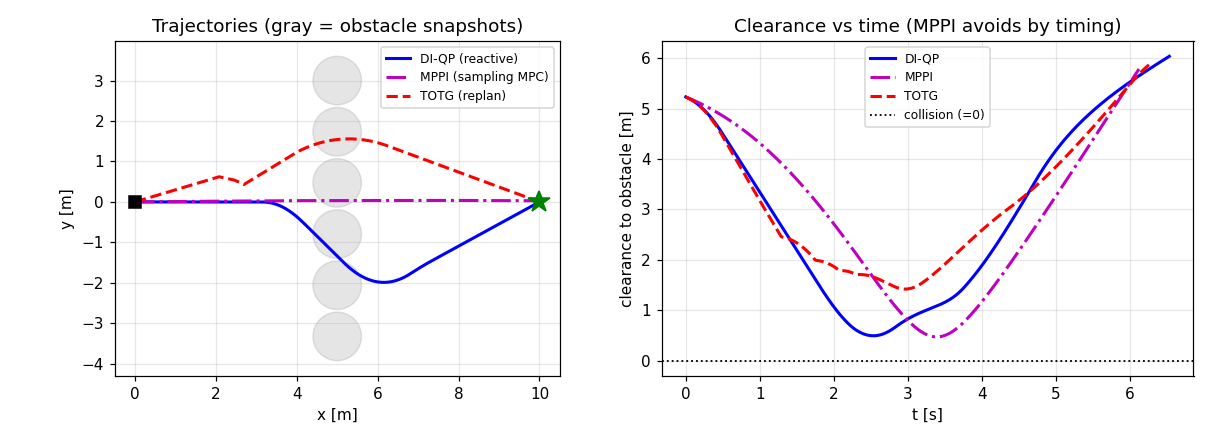
\includegraphics[width=\linewidth]{simulationResults/dynamic_obstacle.png}
\caption{Planar dynamic-obstacle test. Left: trajectories---DI-QP (solid)
detours spatially, MPPI (dash-dot) avoids by \emph{timing} its passage,
path-first (dashed) halts and rebuilds; gray disks are obstacle snapshots.
Right: clearance vs time, all three collision-free. DI-QP reacts without a
path rebuild; across three workstation runs its mean cycle latency is
0.118--0.130 ms versus 1.886--1.979 ms for MPPI, which also lacks hard limits
(Table~\ref{tab:mppi-compare}).}
\label{fig:dynamic-obstacle}
\end{figure}

\subsection{APF Local-Minimum Failure and Waypoint-Injection
Recovery}\label{e.-apf-local-minimum-failure-and-waypoint-injection-recovery}

The APF method is intentionally presented as a soft, high-throughput
heuristic rather than a collision-certificate method. To expose its
failure mode, we place a planar double-integrator robot, goal, and
circular obstacle on the same line. With a purely radial APF field, the
attractive and repulsive terms balance in front of the obstacle and the
planner stalls. A simple waypoint-injection rule detects lack of
progress and inserts a lateral detour sequence around the obstacle; the
same box-constrained QP then reaches the goal while preserving velocity
and acceleration bounds (\texttt{apf\_local\_minimum.py}). Pure APF stalls
6.07 m from the goal (final time 17.99 s), whereas waypoint injection
reaches it (0.12 m residual, 15.56 s) at the same 0.22 m obstacle clearance
and within the same 1.50 m/s and 3.00 m/s² limits, at negligible extra
solve cost (0.135 vs 0.092 ms mean).

This benchmark motivates the hybrid recommendation used throughout the
paper: APF reference deflection is useful for fast reactive steering,
but hard polytope constraints or explicit waypoint/safe-corridor logic
should be activated when progress stalls or clearance must be certified.

\subsection{Scaling to the 7-DOF Arm with a Dynamic
Obstacle}\label{f.-scaling-to-the-7-dof-arm-with-a-dynamic-obstacle}

We exercise the full Section IV machinery on the 7-DOF FR3, where
obstacle constraints couple the joints through the translational
Jacobian. The arm reaches a joint-space goal while a spherical obstacle
crosses the end-effector path. We compare against a
resolved-rate-plus-APF reactive controller without hard limits.

Both avoid the obstacle and reach the goal. The reactive
baseline---lacking hard constraints---exceeds the joint velocity limit at
42 samples and acceleration at 346, whereas the QP holds every joint limit
exactly and keeps the linearized half-space feasible (zero slack), at a
min EE clearance of 0.296 m versus 0.339 m for the unconstrained baseline.
The fixed-sparsity OSQP update path
(\texttt{fixed\_sparsity\_timing.py}) gives the repeated solve and full-cycle
ranges reported in Section~\ref{b.-fr3-manipulator-results}. The single-thread
Python harness meets 100 Hz at p95; full-cycle maxima of 12.26--18.48 ms
identify the tail-latency target for a compiled implementation with reusable
active-set or factorization state.

\begin{figure}[t]
\centering
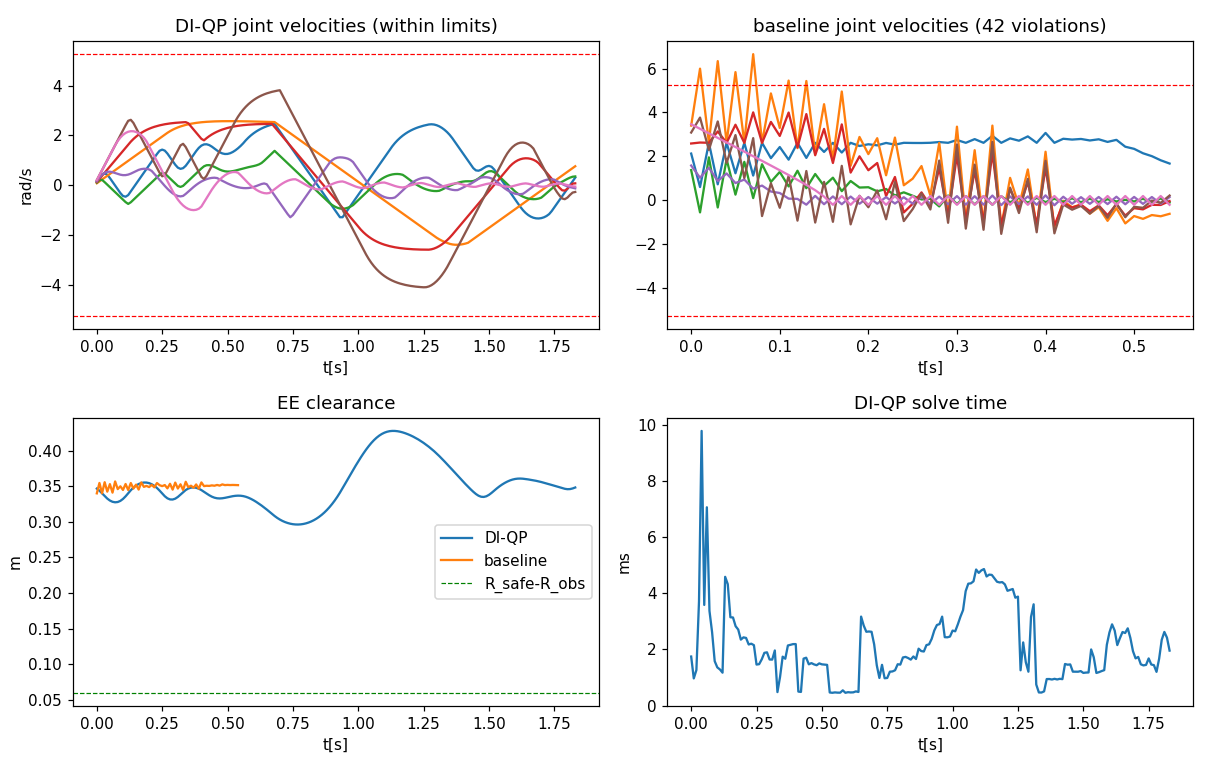
\includegraphics[width=\linewidth]{simulationResults/fr3_dynamic.png}
\caption{7-DOF FR3 dynamic obstacle. Top-left: DI-QP
joint velocities, all within the limit. Top-right: resolved-rate+APF
baseline, which exceeds the velocity limit. Bottom-left: end-effector
clearance. Bottom-right: DI-QP per-cycle solve time.}
\label{fig:fr3-dynamic}
\end{figure}

\subsection{Randomized FR3 Dynamic-Obstacle
Robustness}\label{g.-randomized-fr3-dynamic-obstacle-robustness}

To check that the dynamic-obstacle result is not tied to a single
hand-picked configuration, we perturb the start and goal joint states,
obstacle lateral offset, initial height, and crossing speed over 20
randomized trials (\texttt{fr3\_dynamic\_randomized.py}, seed 7). Both
planners reach the goal in all trials and avoid the obstacle. The
distinction is constraint fidelity: the QP maintains hard joint limits
in every trial, while the resolved-rate baseline repeatedly exceeds
them.

{% converted Pandoc table
\begin{table}[t]
\caption{Randomized FR3 Dynamic-Obstacle Robustness}
\label{tab:fr3-randomized}
\centering
\footnotesize
\setlength{\tabcolsep}{3pt}
\begin{tabular}{@{}>{\raggedright\arraybackslash}p{0.46\linewidth}rr@{}}
\toprule\noalign{}
Metric & DI-QP & Reactive baseline \\
\midrule\noalign{}
Success rate & 100\% & 100\% \\
Min EE clearance, mean ± std {[}m{]} & 0.293 ± 0.018 & 0.328 ± 0.021 \\
Worst min EE clearance {[}m{]} & 0.261 & 0.266 \\
Total joint velocity violations & \textbf{0} & 618 \\
Total joint acceleration violations & \textbf{0} & 6889 \\
Max slack used {[}m{]} & 0.0000 & --- \\
QP solve p95 / max {[}ms{]} & 6.15--6.66 / 25.96--33.10 & --- \\
\bottomrule\noalign{}
\end{tabular}
\end{table}
}

The baseline tends to keep slightly larger clearance because it is
unconstrained and can command arbitrarily aggressive joint velocities
and accelerations. The QP accepts a smaller but still positive clearance
while preserving every declared joint limit.

The timing measurements cover different scopes. The repeated fixed-sparsity
study gives 8.34--9.19 ms solve maxima and 12.26--18.48 ms full-cycle maxima;
across three runs of the 20-trial randomized study, solve p95 is
6.15--6.66 ms and the maximum is 25.96--33.10 ms. The p95 remains below
10 ms, while the full-cycle and randomized maxima locate the tail that a
hard-deadline implementation must reduce.

\subsection{Closed-Loop Dynamics Simulation in
MuJoCo}\label{h.-physical-execution-in-mujoco}

To verify that planner-level differences survive contact with rigid-body
dynamics, we execute both references on a torque-controlled FR3 in
MuJoCo (3.8.1; full mass matrix and gravity). A \(500\) Hz
computed-torque controller tracks each \(100\) Hz reference on the
acute-corner maneuver.

{% converted Pandoc table
\begin{table}[t]
\caption{MuJoCo Computed-Torque Execution}
\label{tab:mujoco-execution}
\centering
\footnotesize
\setlength{\tabcolsep}{3pt}
\begin{tabular}{@{}lcc@{}}
\toprule\noalign{}
Metric (joint 1 / worst) & DI-QP & TOTG \\
\midrule\noalign{}
Peak demanded torque {[}Nm{]} & 58.0 & 56.7 \\
Torque-rate RMS {[}Nm/s{]} & \textbf{181} & 383 \\
Samples over torque limit & 0 & 0 \\
Tracking RMSE {[}mrad{]} & 1.9 & 2.0 \\
\bottomrule\noalign{}
\end{tabular}
\end{table}
}

Both stay within the torque envelope and track to \(\approx 2\) mrad RMS.
TOTG's acceleration discontinuity at the blend seam manifests in simulation as
a stepped torque command (torque-rate RMS \(2.1\times\) that of the DI
reference), while the DI reference produces a smooth torque profile. TOTG
completes the fixed path faster; the DI command is gentler on the
drivetrain---the smoothness-versus-time trade-off in closed-loop dynamics
rather than at the planner output.

\section{Implementation Notes}\label{vii.-implementation-notes}

The QP is solved with OSQP \cite{osqp}. \textbf{Warm-starting} from the
previous solution \(U^*\) cuts cold-start latency from $\sim$5 ms to under
0.5 ms for the decoupled box-constrained QPs. \textbf{Sparse structure} is
reused: the Hessian \(H\) is assembled once offline, the decoupled OSQP
object is set up once with only vectors updated online, and the
coupled-obstacle half-space uses a fixed sparsity pattern updated in place
via OSQP's \texttt{Ax} path, avoiding symbolic re-factorization each cycle.
For \textbf{horizon length}, \(N = 10\) (0.1 s) is too short for pure
position-tracking waypoints, so the default is \(N = 20\) (0.2 s); it
recovers most achievable speed while keeping the coupled QP within a few
milliseconds p95, whereas \(N \approx 30\) narrows the static
time-optimality gap only at higher jerk and solve time.

For multi-waypoint tasks the goal \(x_{\text{goal}}\) is advanced online as
waypoints are reached (within \(\epsilon_q\)); the receding-horizon
time-domain formulation makes these transitions smooth with no path
splicing or re-initialization. The online cost is dominated by the QP solve
itself (\(nN=140\) variables for the 7-DOF \(N{=}20\) case, 141 with a
shared obstacle slack), since the precomputed \(\Phi,\Gamma\) are formed
once and never rebuilt---the practical payoff of the constant-\(A_d\)
property.

\section{Discussion}\label{viii.-discussion}

The proposed framework unifies trajectory generation and time-domain
constraint enforcement in a single continuously-running optimization loop,
rather than planning in space and then parameterizing in time. The
constant-\(A_d\) property---from the nilpotency of the double-integrator
system matrix---is the enabling insight: it decouples trajectory-prediction
cost from configuration. On the test workstation, the Python implementation
achieves sub-10 ms full-cycle p95, while the reported maxima remain above a
hard 100 Hz deadline.

\subsection{Operating Envelope and Validation Scope}\label{scope-and-limitations}

The evaluated method is a \textbf{local} predictive planner whose operating
envelope has four design conditions. \textbf{(i) Timing objective:} a
pure position-tracking cost regulates like a damped second-order system,
with time-to-goal of \(3\)--\(3.5\times\) TOTG; the analytic
velocity-law reference recovers this to \(1.06\)--\(1.32\times\) at zero
violations, acting as a speed-versus-smoothness selector. \textbf{(ii)
Local linearization regime:} Method-A Jacobian linearization has error that
grows quadratically in joint-speed$\times$horizon
($\approx$10 cm at 50\% speed over 0.2 s), so fast or large-detour motions
need a shorter horizon, an inflated Hessian-bound margin, or nonlinear
rollout checking. \textbf{(iii) APF operating mode:} Method-B can settle at a
local equilibrium; waypoint insertion or Method A is used when continued
progress or a certified clearance is required. \textbf{(iv) Finite
look-ahead:} the \(N = 20\) (0.2 s) horizon covers the tested obstacle speeds;
faster obstacles require a longer horizon or an earlier trigger. A terminal
braking-to-rest safe set supports persistent feasibility. The evidence is
simulation-based: randomized coverage comprises 20 FR3 obstacle trials, and
the MuJoCo study is closed-loop rigid-body simulation rather than hardware.

\subsection{Relationship to Path-First and Path--Velocity
Pipelines}\label{relationship-to-path-first-and-pathvelocity-pipelines}

The path-first baseline (TOTG, TOPP-RA) is time-optimal by construction
and plans the whole path at once, an advantage on static tasks. Its B2/B4
acceleration violations arise from circular-blend geometry, not time
parameterization, and vanish with a \(C^2\) path; the near-reversal
singularity likewise eases once curvature is bounded. The architectural
distinction is that a changed path triggers a batch rebuild and the pipeline
begins from a precomputed geometric path, whereas the time-domain formulation
updates the local trajectory directly. The two are complementary: the
proposed planner trades global time-optimality and full-path lookahead for
feasibility, smoothness, conditioning at degeneracies, and fixed-size reactive
updates.

Industrial stacks such as Apollo separate path from speed planning along a
fixed arc-length \(s\), often with a virtual double-integrator speed model
\(\ddot s=u\) \cite{apollo}, and MoveIt pairs geometric planning with
post-hoc time parameterization. The proposed method extends this
virtual-integrator idea from timing along a fixed path to direct
optimization of \(q(t)\), updating path evolution, timing, kinematic
limits, and local obstacle constraints in one convex QP.

A distinct line of reactive planners trades absolute time-optimality for
high-frequency responsiveness: dynamical-system (DS) modulation
\cite{khansari2012} deflects a closed-form velocity field around
obstacles, recent work pairs a joint-space DS with asynchronously
triggered sampling-based MPC for non-convex obstacles \cite{koptev2024},
and MPPI \cite{williams2017} samples parallel rollouts. A parallel line
keeps a precomputed path but governs the reference passed downstream: the
Path Feasibility Governor \cite{pathfg} selects an auxiliary reference
along the path that a nonlinear MPC is guaranteed to track with recursive
feasibility and stability. The present planner modifies the reference in
the same spirit but dispenses with the path altogether---there is no arc
length to govern---trading that formal feasibility certificate for a
fixed-structure convex QP and configuration-independent precomputation.
The methods expose different guarantee sets: the present convex QP directly
enforces hard joint/velocity/acceleration limits, while DS and sampling-based
methods address broader non-convex avoidance. An asynchronous escape in the spirit of
\cite{koptev2024}, triggered when the QP stalls, is a natural extension of
the hybrid switch in
Section~\ref{b.-artificial-potential-field-target-deflection-soft-constraint}.
GPU batch optimizers operate at a different level: CuRobo
\cite{curobo2023} solves a \emph{batch} global trajectory optimization in
$\approx\!50$ ms on a GPU, complementary to a per-cycle receding-horizon
planner---a natural deployment pairs a CuRobo-style global solver with the
DI-QP for reactive correction. Compared with CHOMP, TrajOpt, nonlinear
MPC, or whole-body MPC \cite{sleiman2021}, which solve harder
physical-dynamics problems, the present method instead treats the local
planner as a virtual trajectory generator with precomputed \(\Phi,\Gamma\):
a configuration-independent parameterization for high-rate replanning, not
a new physical model.

% \subsection{Validation Gaps}\label{validation-gaps}

% Three gaps bound the evidence: validation is simulation-only (a physical
% FR3 moving-obstacle experiment is the key next step); the reactive
% comparison should extend the MPPI and nonlinear-MPC baselines to the
% coupled 7-DOF case and add incremental geometric replanners; and only the
% FR3 dynamic-obstacle experiment currently includes randomized trials, so
% broader statistical validation is still needed.

\section{Conclusion}\label{ix.-conclusion}

This paper presented a time-domain local Predictive Motion Planner on a
virtual double-integrator backbone with constant \(A_d\). Because the
prediction matrices are precomputed, online planning reduces to a
fixed-structure convex QP that directly enforces velocity, acceleration,
and local obstacle constraints while producing \(C^1\) reference
trajectories. The experiments show the trade-off clearly: path-first
TOTG/TOPP pipelines are faster on static paths, while the DI-QP keeps
declared time-domain limits explicit and supports fixed-size reactive updates
without a batch rebuild. Future work will focus on non-convex safe
corridors, and comparisons with online MPC and trajectory optimization.

\begin{thebibliography}{17}

\bibitem{ompl}
I. A. Sucan, M. Moll, and L. E. Kavraki, ``The Open Motion Planning Library,'' \emph{IEEE Robotics \& Automation Magazine}, vol. 19, no. 4, pp. 72--82, 2012.

\bibitem{pham2015}
Q.-C. Pham and O. Stasse, ``Time-optimal path parameterization for redundantly actuated robots: A numerical integration approach,'' \emph{IEEE/ASME Transactions on Mechatronics}, vol. 20, no. 6, pp. 3257--3263, 2015.

\bibitem{phri}
Y. Cao and J. Tang, ``Toward Interaction Dynamics: A Predictive Framework for Safe Physical Human--Robot Interaction,'' \emph{arXiv:2606.08281}, 2026. [Online]. Available: \url{https://arxiv.org/abs/2606.08281}

\bibitem{osqp}
B. Stellato, G. Banjac, P. Goulart, A. Bemporad, and S. Boyd, ``OSQP: An operator splitting solver for quadratic programs,'' \emph{Mathematical Programming Computation}, vol. 12, no. 4, pp. 637--672, 2020.

\bibitem{safe_corridor}
S. Liu \emph{et al.}, ``Planning dynamically feasible trajectories for quadrotors using safe flight corridors in 3-D complex environments,'' \emph{IEEE Robotics and Automation Letters}, vol. 2, no. 3, pp. 1688--1695, 2017.

\bibitem{khatib1986}
O. Khatib, ``Real-time obstacle avoidance for manipulators and mobile robots,'' \emph{International Journal of Robotics Research}, vol. 5, no. 1, pp. 90--98, 1986.

\bibitem{toppra}
H. Pham and Q.-C. Pham, ``A new approach to time-optimal path parameterization based on reachability analysis,'' \emph{IEEE Transactions on Robotics}, vol. 34, no. 3, pp. 645--659, 2018.

\bibitem{khatib1987}
O. Khatib, ``A unified approach for motion and force control of robot manipulators: The operational space formulation,'' \emph{IEEE Journal on Robotics and Automation}, vol. 3, no. 1, pp. 43--53, 1987.

\bibitem{mayne2000}
D. Q. Mayne \emph{et al.}, ``Constrained model predictive control: Stability and optimality,'' \emph{Automatica}, vol. 36, no. 6, pp. 789--814, 2000.

\bibitem{kunz2012}
T. Kunz and M. Stilman, ``Time-optimal trajectory generation for path following with bounded acceleration and velocity,'' in \emph{Robotics: Science and Systems}, 2012.

\bibitem{apollo}
ApolloAuto, ``Apollo: An open autonomous driving platform,'' GitHub repository, \url{https://github.com/ApolloAuto/apollo}, accessed June 17, 2026.

\bibitem{sleiman2021}
J.-P. Sleiman, F. Farshidian, M. V. Minniti, and M. Hutter, ``A unified MPC framework for whole-body dynamic locomotion and manipulation,'' \emph{IEEE Robotics and Automation Letters}, vol. 6, no. 3, pp. 4688--4695, 2021.

\bibitem{khansari2012}
S. M. Khansari-Zadeh and A. Billard, ``A dynamical system approach to realtime obstacle avoidance,'' \emph{Autonomous Robots}, vol. 32, no. 4, pp. 433--454, 2012.

\bibitem{koptev2024}
M. Koptev, N. Figueroa, and A. Billard, ``Reactive collision-free motion generation in joint space via dynamical systems and sampling-based MPC,'' \emph{The International Journal of Robotics Research}, vol. 43, no. 13, pp. 2049--2069, 2024.

\bibitem{williams2017}
G. Williams, N. Wagener, B. Goldfain, P. Drews, J. M. Rehg, B. Boots, and E. A. Theodorou, ``Information-theoretic MPC for model-based reinforcement learning,'' in \emph{IEEE Int. Conf. on Robotics and Automation (ICRA)}, 2017, pp. 1714--1721.

\bibitem{storm2022}
M. Bhardwaj, B. Sundaralingam, A. Mousavian, N. D. Ratliff, D. Fox, F. Ramos, and B. Boots, ``STORM: An integrated framework for fast joint-space model-predictive control for reactive manipulation,'' in \emph{Proc. 5th Conf. on Robot Learning (CoRL)}, PMLR vol. 164, 2022, pp. 750--759.

\bibitem{curobo2023}
B. Sundaralingam, S. K. S. Hari, A. Fishman, C. Garrett, K. Van Wyk, V. Blukis, A. Millane, H. Oleynikova, A. Handa, F. Ramos, N. Ratliff, and D. Fox, ``CuRobo: Parallelized collision-free robot motion generation,'' in \emph{IEEE Int. Conf. on Robotics and Automation (ICRA)}, 2023, pp. 8112--8119.

\end{thebibliography}


\end{document}
